\chapter{実験内容}
\section{モデルによる違い}
 本研究ではMagentaで用意されている2つの学習モデルを用いた。以下に示すモデルを用いて楽曲制作をそれぞれ行い,比較,検証する.\\

\subsection{MelodyRNN}
 MelodeRNNは楽曲のメロディを制作するモデルである.MelodyRNNである3つのモデルを以下に示す.\\
(1)	basic_rnn\\
 前の状態を保持し,これを記憶または忘却する.時系列を学習することにより,次の音の予測を可能にしている.Lookback_rnnとAttention_rnnはこれを基に機能を追加したものである.\\
\begin{figure}[!ht]
    \begin{screen}
    \begin{center}
        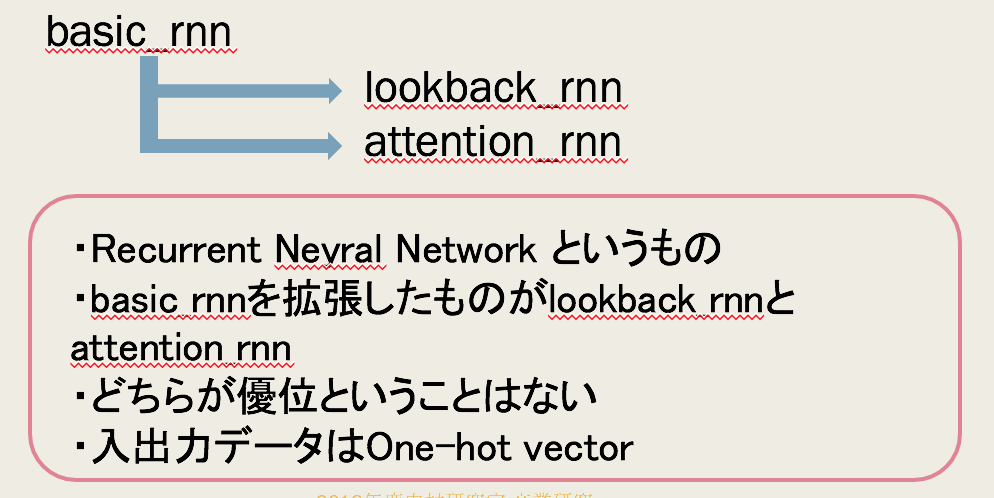
\includegraphics[width=\hsize]{./img/basic1.pdf}
        \caption{magentaによるMIDI音楽データ生成までのプロセ}
        \label{fig:magentaによるMIDI音楽データ生成までのプロセス}
    \end{center}
    \end{screen}
\end{figure}
(2)	lookback_rnn\\
 Basic_rnnを基に,1小節前と2小節前の音,拍数,前の小節の繰り返しかどうかの情報を与え,音楽の流れを掴もうとするもの.\\
(3)	attention_rnn\\
 basic_rnnを基に,過去の情報を予測結果に加えてこれによる繰り返しを捉えるもの.\\

\subsection{PolyphonyRNN}
 複数の同時音のモデリングが可能になっており,複数音の響きを1つのかたまりとして捉えて学習しているモデルである.このモデルを使用することで,伴奏も含めた楽曲の生成が可能である。\\

\section{学習回数による違い}
\section{ノード数による違い}